\documentclass[11pt,a4paper]{article}
%%%%%%%%%%%%%%%%%%%%%%%%% Credit %%%%%%%%%%%%%%%%%%%%%%%%

% template ini dibuat oleh martin.manullang@if.itera.ac.id untuk dipergunakan oleh seluruh sivitas akademik itera.

%%%%%%%%%%%%%%%%%%%%%%%%% PACKAGE starts HERE %%%%%%%%%%%%%%%%%%%%%%%%
\usepackage{graphicx}
\usepackage{caption}
\captionsetup[figure]{name=Gambar}
\usepackage{tabulary}
% \usepackage{amsmath}
\usepackage{fancyhdr}
% \usepackage{amssymb}
% \usepackage{amsthm}
\usepackage{placeins}
% \usepackage{amsfonts}
\usepackage{graphicx}
\usepackage[all]{xy}
\usepackage{tikz}
\usepackage{verbatim}
\usepackage[left=2cm,right=2cm,top=3cm,bottom=2.5cm]{geometry}
\usepackage{hyperref}
\hypersetup{
    colorlinks,
    linkcolor={red!50!black},
    citecolor={blue!50!black},
    urlcolor={blue!80!black}
}
\usepackage{libertine}
\usepackage{libertinust1math}
\usepackage[T1]{fontenc}
\usepackage{inconsolata}

\usepackage{caption}
\usepackage{subcaption}
\usepackage{multirow}
\usepackage{psfrag}
\usepackage[T1]{fontenc}
\usepackage[scaled]{beramono}
% Enable inserting code into the document
\usepackage{listings}
\usepackage{xcolor} 
% custom color & style for listing
\definecolor{codegreen}{rgb}{0,0.6,0}
\definecolor{codegray}{rgb}{0.5,0.5,0.5}
\definecolor{codepurple}{rgb}{0.58,0,0.82}
\definecolor{backcolour}{rgb}{0.95,0.95,0.92}
\lstdefinestyle{mystyle}{
	backgroundcolor=\color{backcolour},   
	commentstyle=\color{green},
	keywordstyle=\color{codegreen},
	numberstyle=\tiny\color{codegray},
	stringstyle=\color{codepurple},
	basicstyle=\ttfamily\footnotesize,
	breakatwhitespace=false,         
	breaklines=true,                 
	captionpos=b,                    
	keepspaces=true,                 
	numbers=left,                    
	numbersep=5pt,                  
	showspaces=false,                
	showstringspaces=false,
	showtabs=false,                  
	tabsize=2
}
\lstset{style=mystyle}
\renewcommand{\lstlistingname}{Kode}
%%%%%%%%%%%%%%%%%%%%%%%%% PACKAGE ends HERE %%%%%%%%%%%%%%%%%%%%%%%%


%%%%%%%%%%%%%%%%%%%%%%%%% Data Diri %%%%%%%%%%%%%%%%%%%%%%%%
\newcommand{\stuid}{120140141}
\newcommand{\student}{\textbf{Bilhaq Avi Dewantara (\stuid{})}}
\newcommand{\course}{\textbf{Sistem Operasi (IF2223)}}
\newcommand{\assignment}{\textbf{02}} % tugas ke...

%%%%%%%%%%%%%%%%%%% using theorem style %%%%%%%%%%%%%%%%%%%%
\newtheorem{thm}{Theorem}
\newtheorem{lem}[thm]{Lemma}
\newtheorem{defn}[thm]{Definition}
\newtheorem{exa}[thm]{Example}
\newtheorem{rem}[thm]{Remark}
\newtheorem{coro}[thm]{Corollary}
\newtheorem{quest}{Question}[section]
%%%%%%%%%%%%%%%%%%%%%%%%%%%%%%%%%%%%%%%%
\usepackage{lipsum}%% a garbage package you don't need except to create examples.
\usepackage{fancyhdr}
\usepackage[ddmmyyyy]{datetime}
\pagestyle{fancy}
\lhead{ \student }
\rhead{ \thepage}
\cfoot{\textbf{Hands On 2: Synchronisation and Deadlock}} % ini untuk judul tugas
\renewcommand{\headrulewidth}{0.4pt}
\renewcommand{\footrulewidth}{0.4pt}

%%%%%%%%%%%%%%  Shortcut for usual set of numbers  %%%%%%%%%%%

\newcommand{\N}{\mathbb{N}}
\newcommand{\Z}{\mathbb{Z}}
\newcommand{\Q}{\mathbb{Q}}
\newcommand{\R}{\mathbb{R}}
\newcommand{\C}{\mathbb{C}}
\setlength\headheight{14pt}

%%%%%%%%%%%%%%%%%%%%%%%%%%%%%%%%%%%%%%%%%%%%%%%%%%%%%%%555

\begin{document}
\thispagestyle{empty}
\begin{center}
	
\includegraphics[scale = 0.15]{Figure/ifitera-header.png}
	\vspace{0.1cm}
\end{center}
\noindent
% change font family for header section only
%{\fontfamily{LinuxLibertineT-OsF}\large\selectfont 
{\large
\rule{17cm}{0.2cm}\\[0.3cm]
Nama: \student \hfill Tugas Ke: \assignment\\[0.1cm]
Mata Kuliah: \course \hfill Tanggal: \today\\
\rule{17cm}{0.05cm}
\vspace{0.1cm}
}


%%%%%%%%%%%%%%%%%%%%%%%%%%%%%%%%%%%%%%%%%%%%% BODY DOCUMENT %%%%%%%%%%%%%%%%%%%%%%%%%%%%%%%%%%%%%%%%%%%%%
\section{Tujuan Hands On 2}
    Tujuan adanya Hands On kedua adalah untuk memahami bagaimana sistem bersinkronisasi dan permasalahan yang ada, serta juga memahami solusinya saat menjalankan critical section.
	Adapun beberapa implementasi yang diharuskan untun dipahami pada Hands On kedua ini antara lain : \textit{join} menggunakan semaphores, \textit{Binary Semaphores}, 
	\textit{Produces Consumer}, \textit{Reader/Writer Locks}, dan \textit{Dining Philosophers}.


\section{Fork/Join}
\subsection{Source Code}
\begin{lstlisting}[language=C]
	#include <stdio.h>
	#include <stdlib.h>
	#include <pthread.h>
	#include <unistd.h>

	#include "common.h"
	#include "common_threads.h"

	#ifdef linux
	#include <semaphore.h>
	#elif __APPLE__
	#include "zemaphore.h"
	#endif

	sem_t s;

	void *child(void *arg) {
	sleep(2);
	printf("child\n");
	Sem_post(&s); // signal here: child is done
	return NULL;
	}

	int main(int argc, char *argv[]) {
	Sem_init(&s, 0); 
	printf("parent: begin\n");
	pthread_t c;
	Pthread_create(&c, NULL, child, NULL);
	Sem_wait(&s); // wait here for child
	printf("parent: end\n");
	return 0;
	}
	\end{lstlisting}

\subsection{Output}
\begin{figure}[h]
	\centering
	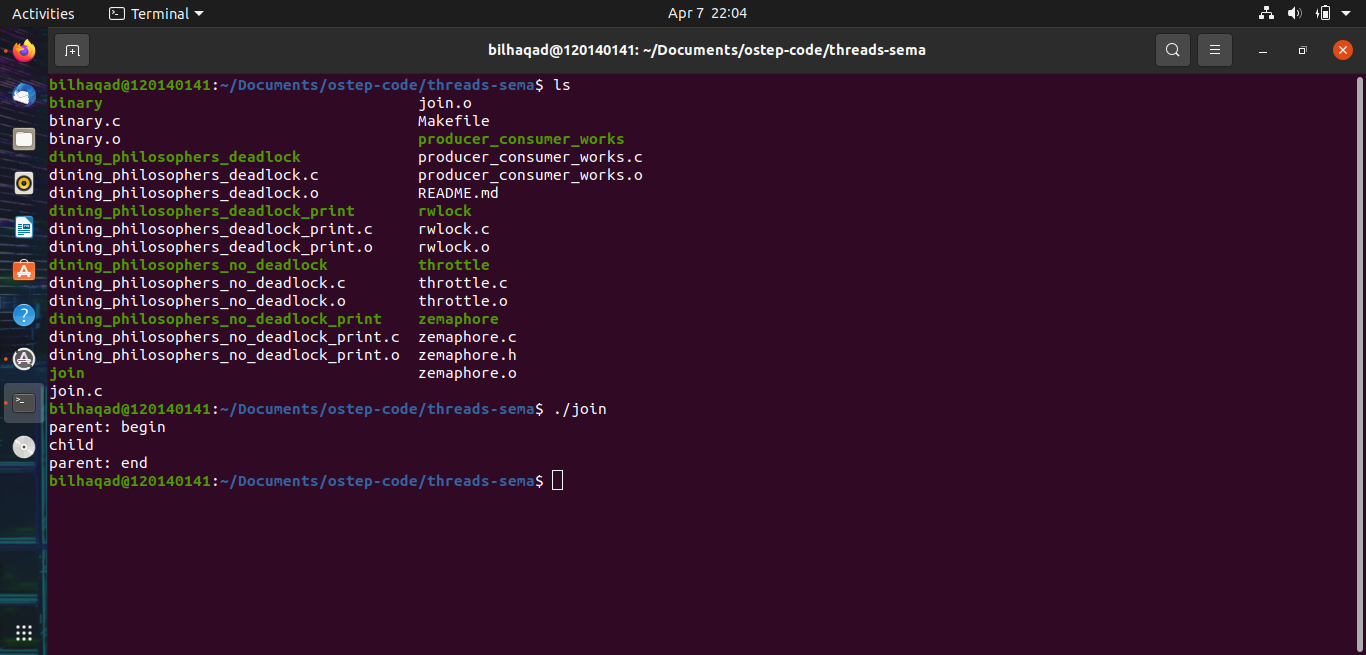
\includegraphics[scale = 0.8]{Figure/fork.png}
	\caption{Fork/Join}
\end{figure}


\section{Pembahasan Tut 1}
\subsection{Tut 1.1 \textit{echo}}
	Pada percobaan tut 1.1 ini akan mencoba perintah \textit{echo} yang akan menampilkan pesan yang kita tuliskan. Pesan yang akan 
	di tulis ialah \textit{"Hello World"}. Dan dengan begitu adanya \textit{echo Hello World}, maka akan mengeluarkan \textit{Hello World} 
	di dalam terminal Linux.
	

\subsection{Tut 1.2 \textit{man}}
    Pada percobaan tut 1.2 ini akan mencoba perintah \textit{man}, dengan mengetik perintah \textit{man echo} di terminal, maka akan 
	mengeluarkan fungsi-fungsi dari sebuah \textit{command man} yang berguna dalam menampilkan sebuah fungsi. Dan dengan adanya \textit{man echo},
	maka akan menampilkan berbagai perintah dan kegunaan dari perintah echo yang dijelaskan secara mendetail.
	

\subsection{Tut 1.3 \textit{echo SHELL}}
	Pada percobaan tut 1.3 ini akan mencoba perintah \textit{echo SHELL} yang akan menampilkan pesan yang kita tuliskan. Pesan yang akan
	di tampilkan dari perintah tersebut ialah mengeluarkan directory \textit{/bin/bash} pada layar terminal.
	

\subsection{Tut 1.4 \textit{who, cd, mkdir, touch, ls, cp, rm}}
	Pada percobaan tut 1.4 ini akan mencoba perintah \textit{who}, \textit{cd}, \textit{mkdir}, \textit{touch}, \textit{ls}, \textit{cp}, 
	\textit{rm} yang akan menampilkan informasi tentang \textit{user}, \textit{directory}, membuat \textit{directory}, membuat file, menampilkan file, 
	menyalin file, dan menghapus file.
	

\newpage
\section{Pembahasan Tut 2}
\subsection{Tut 2.1 \textit{sed}}
	Pada percobaan tut 2.1 ini akan mencoba perintah \textit{sed} yang diminta untuk menghapus 1 karakter di depan dan dibelakang
	di setiap baris code. Sebelumnya saya mencoba untuk membuat file \textit{testing.txt} yang digunakan sebagai tempat eksekusi \textit{sed}.
	Kemudian, barulah saya membuka terminal untuk mulai proses menghapus karakternya dengan perintah \textit{sed} seperti di gambar.
	

\subsection{Tut 2.2 \textit{grep}}
	Pada percobaan tut 2.2 ini akan mencoba perintah \textit{grep} yang diminta untuk mencari karakter tertentu pada sebuah file.
	Sebelumnya saya membuat file \textit{testing.txt} yang digunakan sebagai tempat eksekusi \textit{grep}. Kemudian, barulah saya membuka terminal 
	untuk mulai proses pencarian kata \textit{saya} pada file \textit{testing.txt} seperti yang digambar.
	

\section{Pembahasan Tut 3}
\subsection{Tut 3.1 \textit{Shell Scripting}}
	Pada percobaan tut 3.1 ini akan mencoba perintah \textit{nano} untuk membuat file \textit{test.sh} yang digunakan sebagai tempat mengisi
	kata \textit{echo Hello World}. Selanjutnya, untuk me-\textit{run} file tersebut diperlukan mengetik \textit{chmod +x test.SH} di terminal. Barulah 
	selanjutnya saya mengetik \textit{./test.sh} di terminal untuk menjalankannya.
	

\section{\textit{Assingment 6}}
\subsection*{Source Code}
\begin{lstlisting}[language=bash]
		#get filename
		echo -n "Nama file : "
		read bilhaqavidewantara

		if [!-f $bilhaqavidewantara]
		then
		echo "Nama File $bilhaqavidewantara dosen not exist"
		exit 1
		fi
		tr '[a-z]' '[A-Z]' < $bilhaqavidewantara 
	\end{lstlisting}
	
\subsection*{Penjelasan}
	Pada percobaan \textit{Assignment 6} ini akan mencoba perintah untuk mengubah kalimat yang awalnya berhuruf kecil menjadi 
	kalimat berhuruf besar semua. Pertama saya membuat file \textit{Handson1\_6\_120140141.sh} berisi kode seperti gambar.
	Setelah itu, diperlukan membuat file \textit{test\_6.sh} yang berisi string bebas, dalam hal ini saya isi file tersebut dengan 
	\textit{"bilhaq avi dewantara"}. Kemudian, barulah membuka terminal untuk mengeksekusi program tersebut.
	Pastikan kedua file sudah berada di \textit{directory} yang sama agar memudahkan.
	
	
\section{Assignment 8}
\subsection*{Source Code}
\begin{lstlisting}[language=bash]
		echo "Input nama file : "
		read fname
		echo "Input line pertama yang ingin di output : "
		read s
		echo "Input line terakhir yang ingin di output : "
		read n
		sed -n $s,$n\p $fname | cat > newline
		cat newline
\end{lstlisting}

\subsection*{Penjelasan}
	Pada percobaan \textit{Assignment 8} ini akan mencoba untuk menampilkan baris kalimat yang ingin di \textit{output} dari file.
	Pertama saya membuat file \textit{Handson1\_8\_120140141.sh} berisi kode seperti gambar. Setelah itu, diperlukan membuat file \textit{test\_8.sh}
	untuk membuat kata-kata sebagai \textit{input}. Untuk menjalankannya kita perlu membuka terminal dan user diminta untuk memasukkan 
	baris awal yang akan di \textit{output} dan baris akhir yang akan di \textit{output} pada layar terminal.

\newpage
\section{Assignment 9}
\subsection*{Source Code}
\begin{lstlisting}[language=bash]
		echo "Masukkan kata untuk mencocokkan isi dalam file : "  
		read pat  
		for file in $@  
		do  
			if ! [ -r $file ]  
			then  
				echo "File tidak ada atau tidak terbaca!"  
				continue  
			fi  
			echo "Sebelum -------------------------"  
			cat $file  
			sed -i "/$pat/d" $file  
			echo "Sesudah --------------------------"  
			cat $file  
		done
\end{lstlisting}

\subsection*{Penjelasan}
	Pada percobaan \textit{Assignment 9} ini akan mencoba untuk menghapus baris kalimat yang mengandung kata yang dicari.
	Pertama saya membuat file \textit{Handson1\_9\_120140141.sh} berisi kode seperti gambar. Setelah itu, diperlukan membuat file \textit{test\_9.sh}
	untuk membuat kata-kata sebagai \textit{input}. Untuk menjalankannya kita perlu membuka terminal dan \textit{user} diminta untuk memasukkan 
	kata untuk mencocokkan baris yang ingin di hapus dan akan di \textit{output} pada layar terminal. Pada kode kali ini menggunakan 
	implementasi perintah \textit{echo, read, for, do, if, then, continue, fi, cat, dan sed}.

\newpage
\section{Kesimpulan}
	Pada Hands On 1 ini yang saya dapatkan setelah menjalankannya ialah saya dapat mengenal sistem operasi linux
	khususnya Ubuntu 20.04 LTS ini meskipun hanya menggunakan Oracle VirtualBox. Selain itu, saya dapat mengetahui
	banyak hal dari tugas ini yaitu itu menggunakan konsep-konsep baru dan mengimplementasikannya pada terminal di linux.
	Dengan begitu, saya dapat menyelesaikan tugas ini sesuai dengan kemampuan yang saya miliki terutama menggunakan latex
	ini yang baru bagi saya, sehingga banyak sekali yang saya dapatkan dari tugas ini.
		
\section{Link GitHub}
	Link GitHub dari Hands On 1 ini : \href{https://github.com/BilhaqAD07/Sistem-Operasi.git}{Klik disini}


\newpage
\bibliographystyle{IEEEtran}
\bibliography{Referensi}
\end{document}